\documentclass[twoside]{article}
\usepackage[top=1in, left=0.5in, right=0.5in, bottom=0.5in,paperheight=8.5in,paperwidth=5.5in]{geometry}
\setcounter{secnumdepth}{5}
\setcounter{tocdepth}{5}
\usepackage[english]{babel}
\usepackage{textcomp}
\usepackage[fit]{truncate}
\usepackage{fancyhdr}
\pagestyle{fancy}
\renewcommand{\sectionmark}[1]{\markboth{#1}{}}
\fancyhead{}
\fancyhead[OR]{\leftmark \hspace{0.1cm}  $\vert$ \hspace{0.1cm}  \thepage}
\fancyhead[EL]{\thepage \hspace{0.1cm} $\vert$ \hspace{0.1cm} \leftmark}
\fancyfoot[C]{}%hide footer
\usepackage[hidelinks,plainpages=false]{hyperref}
\usepackage{bibentry}
\usepackage{amsmath,amsthm,amsfonts,amssymb,epsfig}
\usepackage{array}
\usepackage{datetime}
\usepackage{lipsum}% http://ctan.org/pkg/lipsum
\usepackage{listings}% http://ctan.org/pkg/listings
\usepackage{spverbatim}
\usepackage{hyperref}
\usepackage{xcolor} 
\usepackage[scaled=1]{couriers}
\xdefinecolor{gray}{rgb}{0.6,0.6,0.6} 
\Urlmuskip=0mu plus 1mu\relax %needed to make long URLs break nicely
\usepackage{microtype}
\hypersetup{colorlinks=false}
\usepackage{graphicx}
\graphicspath{ {images/} }
\usepackage{parskip}
\usepackage{titlesec} %used for diminishing heading sizes
\titleformat{\section}{\normalfont\bfseries}{\thesection}{1em}{}
\titlespacing*{\section}{0pt}{*2}{0pt}
\titlespacing*{\subsection}{0pt}{*2}{0pt}
\usepackage[square, sort, comma, numbers]{natbib} %%uses titles for cited references

%\usepackage[square,authoryear,sort&compress]{natbib}
%[square, sort, comma, numbers]{natbib} %%uses titles for cited references

\usepackage{xcolor} 
\usepackage[scaled=1]{couriers}
\usepackage{graphicx}
\xdefinecolor{gray}{rgb}{0.6,0.6,0.6} 
\usepackage{setspace}
\usepackage{adjustbox} 
\usepackage[all]{nowidow} %prevent widows/orphans [all,defaultlines]
\usepackage{standalone}


\titleformat*{\section}{\LARGE\bfseries\sffamily}
\titleformat*{\subsection}{\Large\bfseries\sffamily}
\titleformat*{\subsubsection}{\large\bfseries\sffamily}
\titleformat*{\paragraph}{\large\bfseries\sffamily}
\titleformat*{\subparagraph}{\large\bfseries\sffamily}
\renewcommand{\familydefault}{\sfdefault} %sans-serif font

% TO DO: Find better templates for R and Python



%----------------------------------------------------------------------
% Definition for "lstlisting" blocks
%----------------------------------------------------------------------
% --- USAGE ---
%
% \begin{lstlisting}[style=R}
% ...
% \end{lstlisting}
%
% % \begin{lstlisting}[style=output}
% ...
% \end{lstlisting}
%----------------------------------------------------------------------

% By default, make listings all black so it's easy to spot the ones that aren't set to a style.
% This is just a debugging technique.
%\lstset{backgroundcolor=\color{black}}

% http://latexcolor.com/
\definecolor{deepblue}{rgb}{0,0,0.5}
\definecolor{deepred}{rgb}{0.6,0,0}
\definecolor{deepgreen}{rgb}{0,0.5,0}
%\definecolor{tan}{rgb}{0.98, 0.92, 0.84}  %antiquewhite
%\definecolor{r_bkgd}{rgb}{1.0, 0.92, 0.8}  %blacnedalmond
\definecolor{py_bkgd}{rgb}{0.94, 0.97, 1.0}  %aliceblue
\definecolor{ashgrey}{rgb}{0.7, 0.75, 0.71}
\definecolor{battleshipgrey}{rgb}{0.52, 0.52, 0.51}
%\definecolor{r_bkgd}{rgb}{0.97, 0.91, 0.81}  %champagne
\definecolor{r_bkgd}{rgb}{0.98, 0.92, 0.84}  %moccasin

\definecolor{Code}{rgb}{0,0,0}
\definecolor{Decorators}{rgb}{0.5,0.5,0.5}
\definecolor{Numbers}{rgb}{0.5,0,0}
\definecolor{MatchingBrackets}{rgb}{0.25,0.5,0.5}
\definecolor{Keywords}{rgb}{0,0,1}
\definecolor{self}{rgb}{0,0,0}
\definecolor{Strings}{rgb}{0,0.63,0}
\definecolor{Comments}{rgb}{0,0.63,1}
\definecolor{Backquotes}{rgb}{0,0,0}
\definecolor{Classname}{rgb}{0,0,0}
\definecolor{FunctionName}{rgb}{0,0,0}
\definecolor{Operators}{rgb}{0,0,0}
\definecolor{Background}{rgb}{0.98,0.98,0.98}

% KEYWORDS
% http://tex.stackexchange.com/questions/186092/how-can-i-delete-non-letter-keywords-such-as
\lstdefinestyle{Scala}{
  language={Scala},
  frame=single,
  breaklines,
  basicstyle=\ttfamily,
  commentstyle=\itshape\color{battleshipgrey},% comment style
  %commentstyle=\textsl,% comment style
  %keywordstyle=\ttfamily\color{deepblue},
  %keywordstyle=\color{WildStrawberry},
  numbers=left,% display line numbers on the left side
  numberstyle=\scriptsize,% use small line numbers
  numbersep=10pt,% space between line numbers and code
  backgroundcolor=\color{white},
  showstringspaces=false,
  stringstyle=\color{deepgreen},
  backgroundcolor=\color{py_bkgd},
  % keywords
  morekeywords={abstract,case,catch,class,def,%
    do,else,extends,false,final,finally,%
    for,if,implicit,import,match,mixin,%
    new,null,object,override,package,%
    private,protected,requires,return,sealed,%
    super,this,throw,trait,true,try,%
    type,val,var,while,with,yield},
  otherkeywords={=>,<-,<\%,<:,>:,\#,@},
  sensitive=true,
  morecomment=[l]{//},
  morecomment=[n]{/*}{*/},
  morestring=[b]``,
  morestring=[b]',
  morestring=[b]''``,
  keywordstyle={\color{Keywords}\bfseries},
}

\lstdefinestyle{R}{
  language={R},
  frame=single,
  breaklines,
  basicstyle=\ttfamily,
  %commentstyle=\textsl\color{Comments},% comment style
  commentstyle=\itshape\color{battleshipgrey},% comment style
  keywordstyle=\ttfamily\color{deepblue},
  numbers=left,% display line numbers on the left side 
  numberstyle=\scriptsize,% use small line numbers 
  numbersep=10pt,% space between line numbers and code
  backgroundcolor=\color{r_bkgd},
  showstringspaces=false,
  stringstyle=\color{deepgreen},
  %morekeywords={TRUE, FALSE, for, if},
  keywordstyle={\color{Keywords}\bfseries},
  keywords={TRUE, FALSE},
  deletekeywords={grid, frame, variable, model, vi, predict, file},
  otherkeywords={!,!=,~,$,*,\&,\%/\%,\%*\%,\%\%,<-,<<-},
  %morekeywords={TRUE, FALSE, list, c}
}



\lstdefinestyle{python}{
  language={Python},
  frame=single,
  breaklines,
  basicstyle=\ttfamily,
  commentstyle=\itshape\color{battleshipgrey},% comment style
  %commentstyle=\textsl,% comment style
  %keywordstyle=\ttfamily\color{deepblue},
  %keywordstyle=\color{WildStrawberry},
  numbers=left,% display line numbers on the left side 
  numberstyle=\scriptsize,% use small line numbers 
  numbersep=10pt,% space between line numbers and code
  backgroundcolor=\color{white},
  showstringspaces=false,
  stringstyle=\color{deepgreen},
  backgroundcolor=\color{py_bkgd},
  % keywords
morekeywords={import,from,class,def,for,while,if,is,in,elif,else,not,and,or,print,break,continue,return,True,False,None,access,as,,del,except,exec,finally,global,import,lambda,pass,print,raise,try,assert},
 keywordstyle={\color{Keywords}\bfseries},
}

\lstdefinestyle{Bash}{
  language=bash,
  frame=single,
  breaklines,
  basicstyle=\ttfamily,
  commentstyle=\textsl,% comment style
  keywordstyle=\ttfamily,
  numbers=left,% display line numbers on the left side
  numberstyle=\scriptsize,% use small line numbers
  numbersep=10pt,% space between line numbers and code
  backgroundcolor=\color{white},
  showstringspaces=false % don't show spaces as weird char.
}

\definecolor{mygray}{rgb}{0.92,0.92,0.92}

\lstdefinestyle{output}{
  frame=single,
  breaklines,
  basicstyle=\ttfamily,
  numbers=left,% display line numbers on the left side 
  numberstyle=\scriptsize,% use small line numbers 
  numbersep=10pt,% space between line numbers and code
  backgroundcolor=\color{mygray},
  showstringspaces=false 
}

\newcommand{\waterExampleInR} {
\textbf{Example in R} \\
}

\newcommand{\waterExampleInPython} {
\textbf{Example in Python} \\
}
 %lacks Scala style setup
%
% Use fancy table
%
\usepackage{tabularx}
\usepackage{booktabs}
\usepackage{forest}
\usepackage{url}
\usepackage{longtable}
\def\UrlBreaks{\do\/\do-\do_\do.}

\begin{document}

\thispagestyle{empty} %removes page number  

\begin{center}
\textsc{\large\bf{Machine Learning with Sparkling Water: H2O + Spark}}

\bigskip
\line(1,0){250}  %inserts  horizontal line 
\\
\bigskip
\textsc{\small{Michal Malohlava\hspace{20pt} Jakub Hava\hspace{20pt} Nidhi Mehta}}

\textsc{\small{Edited by: Vinod Iyengar \&\ Angela Bartz}}
\\
\bigskip
\line(1,0){250}  %inserts  horizontal line


{\url{http://h2o.ai/resources}}

\bigskip
\monthname \hspace{1pt}  \the\year: Fourth Edition
\\%add front page image here? (wavy lines)
\bigskip
\end{center}

\newpage
\null\vfill %move next text block to lower left of new page

\thispagestyle{empty}%remove pg#


{\raggedright\vfill\ 

Machine Learning with Sparkling Water: H2O + Spark\\
  by Michal Malohlava, Jakub Hava, \&\ Nidhi Mehta\\
  Edited by: Vinod Iyengar \&\ Angela Bartz
  
\bigskip
  Published by H2O.ai, Inc. \\
2307 Leghorn St. \\
Mountain View, CA 94043\\
\bigskip
\textcopyright 2016-\the\year \hspace{1pt} H2O.ai, Inc. All Rights Reserved. 
\bigskip

\monthname \hspace{1pt}  \the\year: Third Edition
\bigskip

Photos by \textcopyright H2O.ai, Inc. 
\bigskip

While every precaution has been taken in the\\
preparation of this book, the publisher and\\
authors assume no responsibility for errors or\\
omissions, or for damages resulting from the\\
use of the information contained herein.\\
\bigskip
Printed in the United States of America. 


}\par

\newpage
\tableofcontents

\newpage
\documentclass{standalone}

\begin{document}


    \section{What is H2O?}
    \Urlmuskip=0mu plus 1mu\relax %needed to make long URLs break nicely


    H2O.ai focuses on bringing AI to businesses through software.
    Its flagship product is H2O, the leading open-source platform that makes it easy for financial
    services, insurance companies, and healthcare companies to deploy AI and deep learning to solve complex problems.
    More than 9,000 organizations and 80,000+ data scientists depend on H2O for critical applications like predictive
    maintenance and operational intelligence. The company -- which was recently named to the CB Insights AI 100 -- is used
    by 169 Fortune 500 enterprises, including 8 of the world's 10 largest banks, 7 of the 10 largest insurance companies, and
    4 of the top 10 healthcare companies. Notable customers include Capital One, Progressive Insurance, Transamerica, Comcast,
    Nielsen Catalina Solutions, Macy's, Walgreens, and Kaiser Permanente.

    Using in-memory compression, H2O handles billions of data rows in-memory, even with a small cluster. To make it easier
    for non-engineers to create complete analytic workflows, H2O's platform includes interfaces for R, Python, Scala, Java,
    JSON, and CoffeeScript/JavaScript, as well as a built-in web interface, Flow. H2O is designed to run in standalone
    mode, on Hadoop, or within a Spark Cluster, and typically deploys within minutes.

    H2O includes many common machine learning algorithms, such as generalized linear modeling (linear regression, logistic
    regression, etc.), Na\"{i}ve Bayes, principal component analysis, k-means clustering, and word2vec. H2O implements
    best-in-class algorithms at scale, such as distributed random forest, gradient boosting, and deep learning. H2O also
    includes a Stacked Ensembles method, which finds the optimal combination of a collection of prediction algorithms using
    a process known as "stacking." With H2O, customers can build thousands of models and compare the results to get the
    best predictions.

    H2O is nurturing a grassroots movement of physicists, mathematicians, and computer scientists to herald the new wave
    of discovery with data science by collaborating closely with academic researchers and industrial data scientists.
    Stanford university giants Stephen Boyd, Trevor Hastie, and Rob Tibshirani advise the H2O team on building scalable
    machine learning algorithms. And with hundreds of meetups over the past several years, H2O continues to remain
    a word-of-mouth phenomenon.

    \textbf{Try it out}

    \begin{itemize}
        \setlength\itemsep{1pt}
        \item  Download H2O directly at {\url{http://h2o.ai/download}}.
        \item Install H2O's R package from CRAN at {\url{https://cran.r-project.org/web/packages/h2o/}}.
        \item Install the Python package from PyPI at {\url{https://pypi.python.org/pypi/h2o/}}.

    \end{itemize}


    \begin{minipage}{\textwidth}
        \textbf{Join the community}
        \setlength{\parskip}{1em}
        \begin{itemize}
            \setlength\itemsep{1pt}
            \item To learn about our training sessions, hackathons, and product updates, visit {\url{http://h2o.ai}}.
            \item To learn about our meetups, visit {\url{https://www.meetup.com/topics/h2o/all/}}.
            \item Have questions? Post them on Stack Overflow using the \textbf{h2o} tag at {\url{http://stackoverflow.com/questions/tagged/h2o}}.
            \item Have a Google account (such as Gmail or Google+)? Join the open-source community forum at {\url{https://groups.google.com/d/forum/h2ostream}}.
            \item Join the chat at {\url{https://gitter.im/h2oai/h2o-3}}.
        \end{itemize}
    \end{minipage}

\end{document}


\newpage
\documentclass{standalone}

\begin{document}

\section{Sparkling Water Introduction}

Sparkling Water allows users to combine the fast, scalable machine learning algorithms of H2O with the capabilities of Spark. With Sparkling Water, users can drive computation from Scala, R, or Python and use the H2O Flow UI, providing an ideal machine learning platform for application developers.

Spark is an elegant and powerful general-purpose, open-source, in-memory platform with tremendous momentum. H2O is an in-memory application for machine learning that is reshaping how people apply math and predictive analytics to their business problems.

Integrating these two open-source environments provides a seamless experience for users who want to make a query using Spark SQL, feed the results into H2O to build a model and make predictions, and then use the results again in Spark. For any given problem, better interoperability between tools provides a better experience. 

For additional examples, please visit the Sparkling Water GitHub repository at {\url{https://github.com/h2oai/sparkling-water/tree/master/examples}}.

\begin{minipage}{\textwidth}
    \textbf{Have Questions about Sparkling Water?}
    \setlength{\parskip}{1em}
    \begin{itemize}
        \setlength\itemsep{1pt}
        \item Post them on Stack Overflow using the \textbf{sparkling-water} tag at {\url{http://stackoverflow.com/questions/tagged/sparkling-water}}.
        \item Join the chat at {\url{https://gitter.im/h2oai/sparkling-water}}.
    \end{itemize}
\end{minipage}

\subsection{Typical Use Cases}
Sparkling Water excels in leveraging existing Spark-based workflows needed to call advanced machine learning algorithms. We identified three the most common use-cases which are described below. 

\subsubsection{Model Building}
A typical example involves multiple data transformations with help of Spark API, where a final form of data is transformed into H2O frame and passed to an H2O algorithm. The constructed model estimates different metrics based on the testing data or gives a prediction that can be used in the rest of the data pipeline (see Figure~\ref{fig:uc1}).
\begin{figure}[h!]
	\centering
	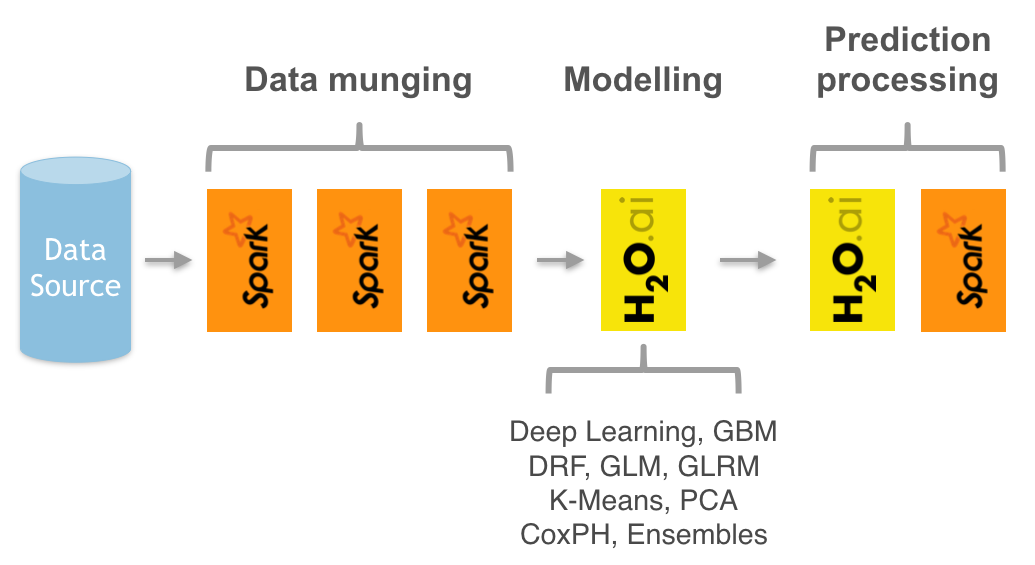
\includegraphics[width=0.9\textwidth]{../images/uc1.png}
	\caption{Sparkling Water extends existing Spark data pipeline with advanced machine learning algorithms.}
	\label{fig:uc1} 
\end{figure}

\subsubsection{Data Munging}
Another use-case includes Sparkling Water as a provider of ad-hoc data transformations. Figure~\ref{fig:uc2} shows a data pipeline benefiting from H2O's parallel data load and parse capabilities, while Spark API is used as another provider of data transformations. Furthermore, H2O can be used as in-place data transformer.

\begin{figure}[h!]
	\centering
	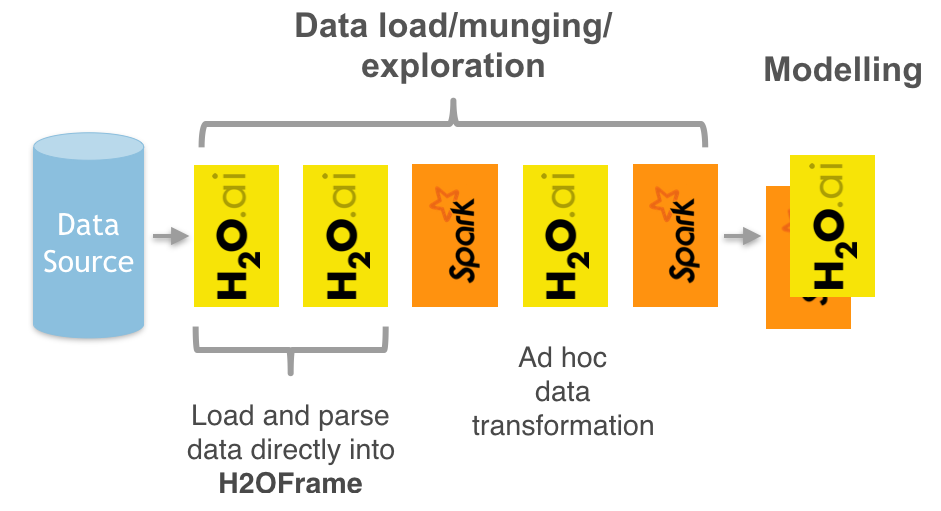
\includegraphics[width=0.9\textwidth]{../images/uc2.png}
	\caption{Sparkling Water introduces H2O parallel load and parse into Spark pipelines.}
	\label{fig:uc2} 
\end{figure}

\subsubsection{Stream Processing}
The last use-case depicted on Figure~\ref{fig:uc3} introduces two data pipelines. The first one, called an off-line training pipeline, is invoked regularly (e.g., every hour or every day), utilizes Spark as well as H2O API and provides an H2O model as output. The H2O API allows the model to be exported in a form independent on H2O run-time. The second one processes streaming data (with help of Spark Streaming or Storm) and utilizes the model trained in the first pipeline to score the incoming data. Since the model is exported with no run-time dependency to H2O, the streaming pipeline can be lightweight and independent on H2O or Sparkling Water infrastructure.

\begin{figure}[h]
	\centering
	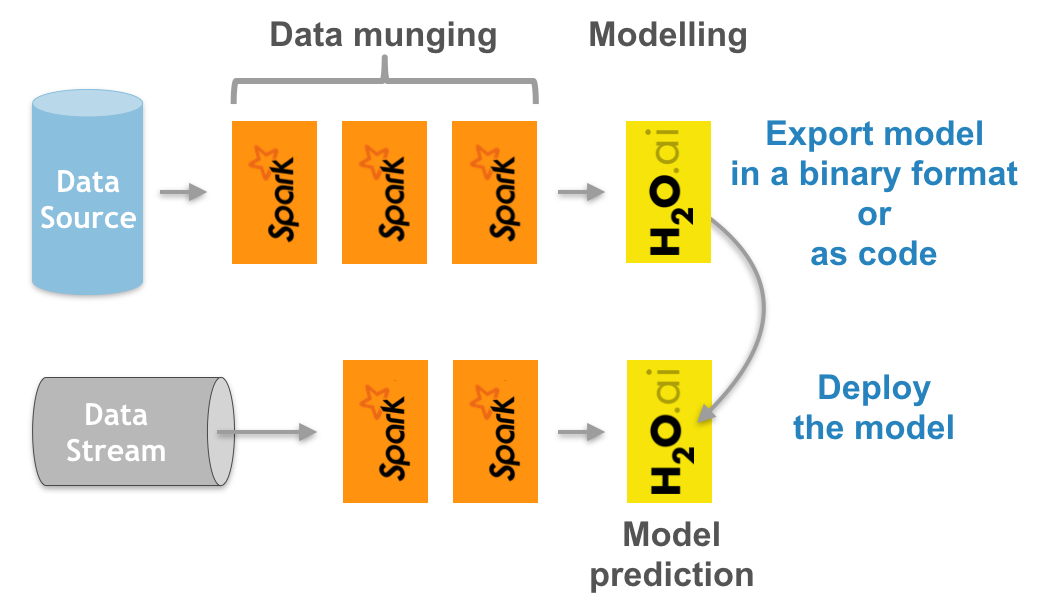
\includegraphics[width=0.9\textwidth]{../images/uc3.png}
	\caption{Sparkling Water used as an off-line model producer feeding models into a stream-based data pipeline.}
	\label{fig:uc3} 
\end{figure}

\subsection{Features}

Sparkling Water provides transparent integration for the H2O engine and its machine learning algorithms into the Spark platform, enabling:

\begin{itemize}

 \item Use of H2O algorithms in Spark workflow
 \item Transformation between H2O and Spark data structures
 \item Use of Spark RDDs, DataFrames and Datasets as input for H2O algorithms
 \item Use of H2OFrames as input for MLlib algorithms
 \item Transparent execution of Sparkling Water applications on top of Spark
 \item Use H2O algorithms in Spark pipelines
\end{itemize}

\subsection{Supported Data Sources}

Currently, Sparkling Water can use the following data source types:

\begin{itemize}

 \item Standard Resilient Distributed Dataset (RDD) API for loading data and transforming it into H2OFrames
 \item H2O API for loading data directly into H2OFrame from file(s) stored on:
  \begin{itemize}
    \item local filesystems
    \item HDFS
    \item S3
    \item HTTP/HTTPS
  \end{itemize}
\end{itemize}

For more details, please refer to the H2O documentation at {\url{http://docs.h2o.ai}}.

\subsection{Supported Data Formats}

Sparkling Water can read data stored in the following formats:

\begin{itemize}

  \item CSV
  \item SVMLight
  \item ARFF
  \item Parquet
\end{itemize}

For more details, please refer to the H2O documentation at {\url{http://docs.h2o.ai}}.

\subsection{Supported Spark Execution Environments}
Sparkling Water can run on top of Spark in the following ways:
\begin{itemize}
  \item as a local cluster (where the master node is \texttt{local} or \texttt{local[*]})
  \item as a standalone cluster\footnote{Refer to the Spark standalone documentation
\url{http://spark.apache.org/docs/latest/spark-standalone.html}} 
\item in a YARN environment\footnote{Refer to the Spark YARN documentation \url{http://spark.apache.org/docs/latest/running-on-yarn.html}}

\end{itemize}
\end{document}



\newpage
\documentclass{standalone}
\usepackage{placeins}
\begin{document}


\section{Design}
Sparkling Water is designed to be executed as a regular Spark application. It provides a way to initialize H2O services on Spark and access data stored in data structures of Spark and H2O.

Sparkling Water supports two type of backends. In the internal backend, Sparkling Water is launched inside
a Spark executor, which is created after application submission. At this point, H2O starts services,
including distributed key-value (K/V) store and memory manager, and orchestrates them into a cloud.
The topology of the created cloud matches the topology of the underlying Spark cluster exactly.
The following figure represents the Internal Sparkling Water cluster.


\begin{figure}[h!]
	\centering
	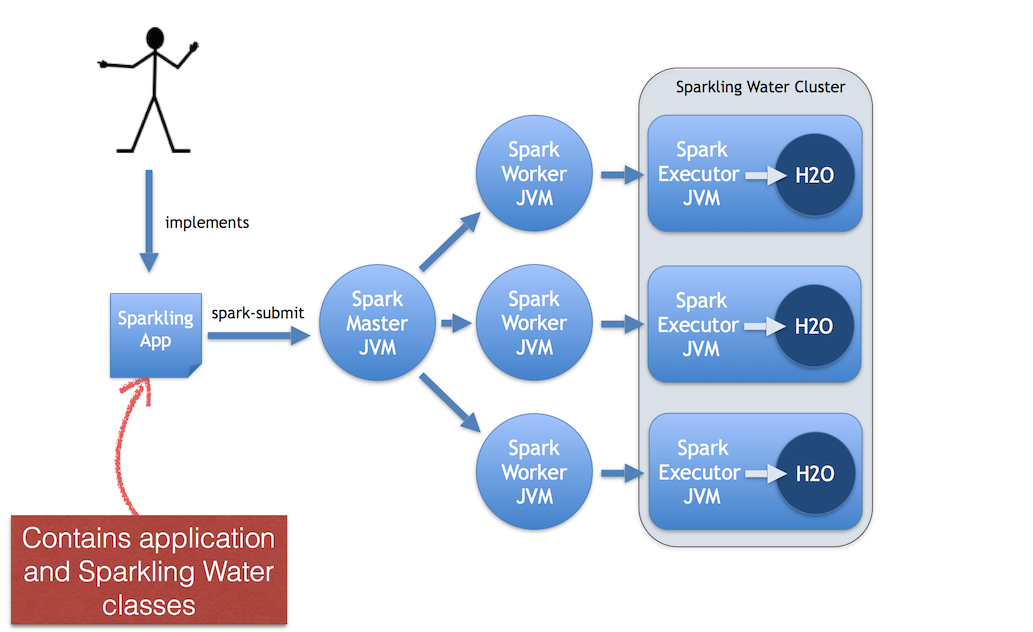
\includegraphics[scale=0.6]{../images/Topology-internal.png}
	\caption{Sparkling Water design depicting deployment of the Sparkling Water in internal backend to the standalone Spark cluster.}
\end{figure}

In external backend, the H2O cluster is started separately and is connected to from the Spark driver. The following figure represents the External Sparkling Water cluster.

\begin{figure}[h!]
	\centering
	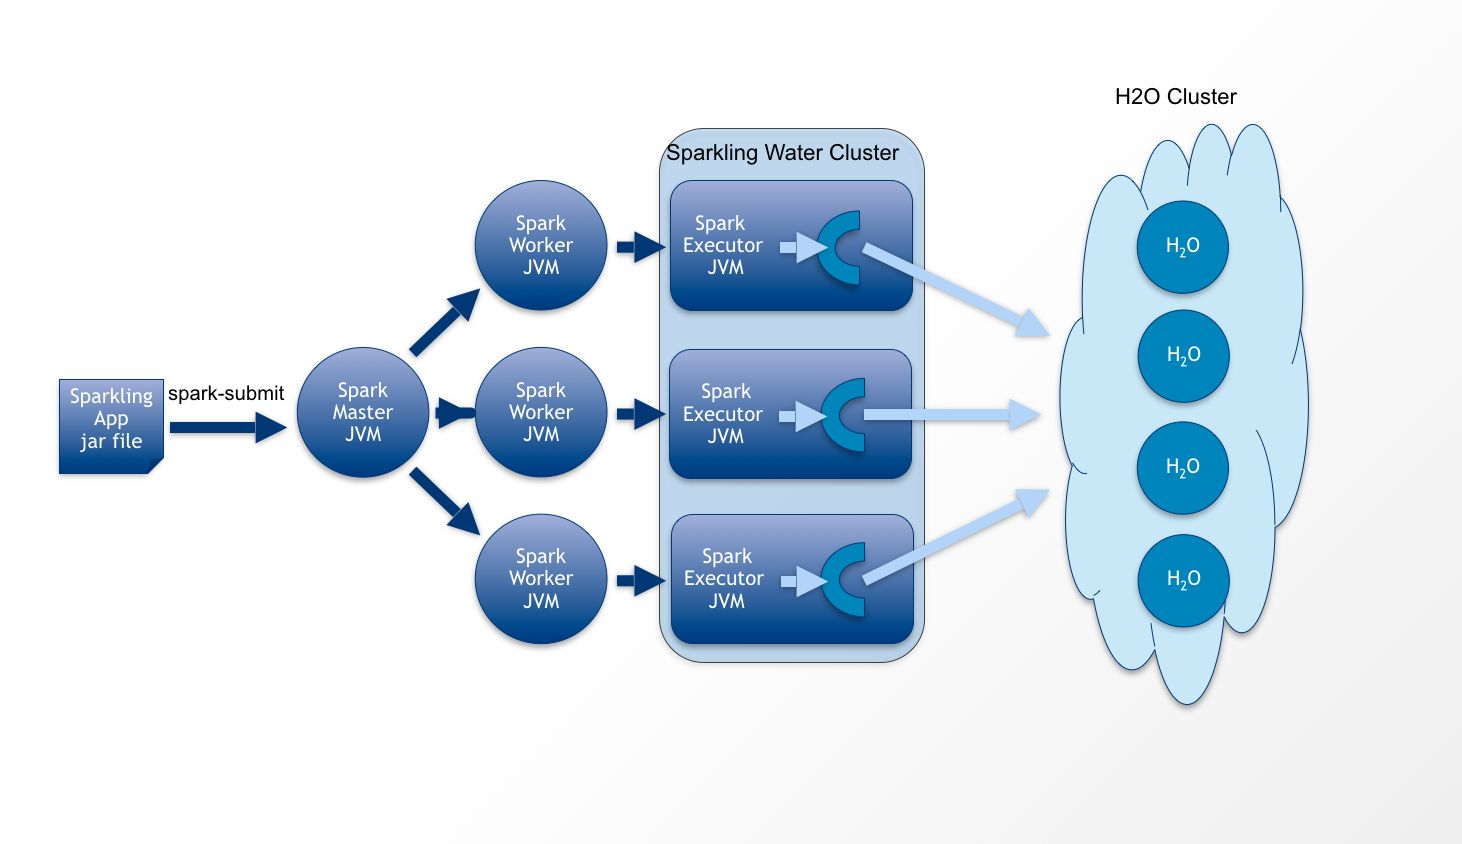
\includegraphics[scale=0.4]{../images/Topology-external.png}
	\caption{Sparkling Water design depicting deployment of the Sparkling Water in internal backend to the standalone Spark cluster.}
\end{figure}

More information about backends is available in the next section.

\subsection{Data Sharing between Spark and H2O}

Sparkling Water enables transformation between different types of RDDs and H2O's \texttt{H2OFrame}, and vice versa.

When converting from an \texttt{H2OFrame} to an RDD, a wrapper is created around the \texttt{H2OFrame} to provide an RDD-like API. In this case,  data is not duplicated but served directly from the underlying \texttt{H2OFrame}.

Converting from an RDD/DataFrame to an \texttt{H2OFrame} requires data duplication because it transfers data from the RDD storage into \texttt{H2OFrame}. However, data stored in an \texttt{H2OFrame} is heavily compressed and does not need to be preserved in RDD.

\begin{figure}[h!]
	\centering
	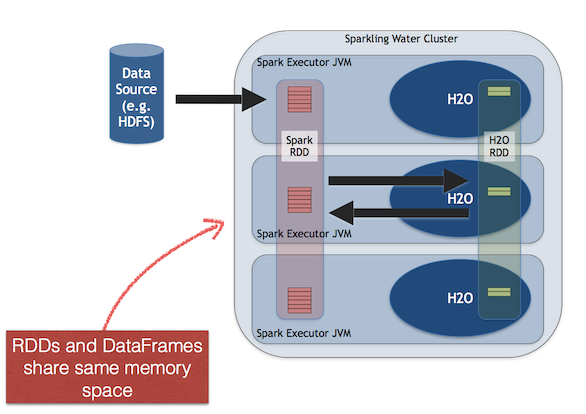
\includegraphics[scale=1]{../images/DataShare.png}
	\caption{Sharing between Spark and H2O inside an executor JVM.}
\end{figure}

\subsection{Provided Primitives}

Sparkling Water provides several primitives (Table~\ref{tab:primitives}), which are the basic components used by Spark components.

\begin{table}[!ht]
	\centering
	%\begin{adjustbox}{width=\textwidth} %resizes table to text width
	%\setlength{\tabcolsep}{2pt} %narrow column separation
	\begin{tabular}{c c p{5.2cm}}
		%\begin{tabularx}{\textwidth}{l l p{5.2cm}}
		\toprule
		Concept & API Implementation& Description \\
		\midrule
		H2O Context & \texttt{H2OContext} & Contains
		H2O and Sparkling Water state, provides primitives to publish data in Spark as \texttt{H2OFrame} and
		vice versa. It follows design principles of Spark primitives such as
		\texttt{SparkSession}, \texttt{SparkContext} or \texttt{SQLContext}. \\ \addlinespace
		%\small{(Full name: \small{\texttt{org.apache.spark.\break h2o.H2OContext}}}) \\  \addlinespace

		H2O Entry Point & \texttt{water.H2O} & Represents the entry point for accessing
		H2O services. Contains information about running H2O services, including a list of
		nodes and the status of the distributed K/V datastore. \\  \addlinespace

		H2O Frame &  \small{\texttt{water.fvec.H2OFrame}} & A distributed data structure
		representing a table of values. The table is column-based and provides column and
		row accessors. \\  \addlinespace

		H2O Algorithm & package \texttt{hex} & Represents the H2O machine learning
		algorithms library, including DeepLearning, GBM, GLM, DRF, and other
		algorithms. \\

		\bottomrule
	\end{tabular}
	%\end{tabularx}
	\caption{Sparkling Water primitives}
	\label{tab:primitives}
\end{table}

Before using H2O algorithms and data structures, the first step is to create and start the \texttt{H2OContext} instance using the \\
\texttt{val hc = new H2OContext.getOrCreate(spark)} call.
\texttt{H2OContext} contains the necessary information for running H2O services and exposes methods for data transformation between the Spark RDD, \texttt{DataFrame} or \texttt{Dataset}, and the \texttt{H2OFrame}.
Starting \texttt{H2OContext} involves an operation that:

\begin{itemize}
 \item In case of internal backend, is distributed and contacts all accessible Spark executor nodes and initializes H2O services (such as the key-value store and RPC) inside the executors' JVMs.
 \item In case of external backend, either starts H2O cluster on YARN and connects to it or connects to existing H2O cluster right away (depends on the configuration).
\end{itemize}

\newpage
When \texttt{H2OContext} is running, H2O data structures and algorithms can be manipulated. The key data structure is \texttt{H2OFrame}, which represents a distributed table composed of vectors. A new \texttt{H2OFrame} can be created using one of the following methods:
\begin{itemize}
	\item loading a cluster local file (a file located on each node of the cluster):
\begin{lstlisting}[style=Scala]
val h2oFrame = new H2OFrame(new File("/data/iris.csv"))
\end{lstlisting}
	\item loading a file from HDFS/S3/S3N/S3A:
\begin{lstlisting}[style=Scala]
val h2oFrame = new H2OFrame(URI.create("hdfs://data/iris.csv"))
\end{lstlisting}
	\item loading multiple files from HDFS/S3/S3N/S3A:
\begin{lstlisting}[style=Scala]
val h2oFrame = new H2OFrame(
    URI.create("hdfs://data/iris/01.csv"),
    URI.create("hdfs://data/iris/02.csv")
)
\end{lstlisting}
	\item transforming Spark RDD, \texttt{DataFrame} or \texttt{Dataset}:
\begin{lstlisting}[style=Scala]
val h2oFrame = h2oContext.asH2OFrame(sparkData)
\end{lstlisting}
	\item referencing existing \texttt{H2OFrame} by its key
\begin{lstlisting}[style=Scala]
val h2oFrame = new H2OFrame("iris.hex")
\end{lstlisting}		
\end{itemize}


When \texttt{H2OContext} is running, any H2O algorithm can be called. Most of the provided algorithms are located in the \texttt{hex} package. Calling an algorithm is composed of two steps:

\begin{itemize}
	\item Specifying parameters:
\begin{lstlisting}[style=Scala]
val train: H2OFrame = new H2OFrame(new File("prostate.csv"))
val gbmParams = new GBMParameters()
gbmParams._train = train
gbmParams._response_column = "CAPSULE"
gbmParams._ntrees = 10
\end{lstlisting}

	\item Creating the model builder and launching computations. The \texttt{trainModel} method is non-blocking and returns a job representing the computation.
\begin{lstlisting}[style=Scala]
val gbmModel = new GBM(gbmParams).trainModel.get
\end{lstlisting}
\end{itemize}

\end{document}


\newpage
\section{Sparkling Water Backends}

\subsection{Internal Backend}

In internal backend, H2O cloud is created automatically during the call of \texttt{H2OContext.getOrCreate}. Since it's not technically possible to get the number of executors in Spark, Sparkling Water tries to discover all executors at the initiation of \texttt{H2OContext} and starts H2O instance inside of each discovered executor. This solution is the easiest to deploy; however when Spark or YARN kills the executor, the whole H2O cluster goes down since H2O doesn't support high availability. The
same happens also for the case when a new executors join the cluster as the shape of the H2O cluster can't be changed later.
Internal backend is default for behaviour for Sparkling Water. It can be changed via spark configuration property
\texttt{spark.ext.h2o.backend.cluster.mode} to \textbf{external} or \textbf{internal}. Another way how to change type of backend is by calling \texttt{setExternalClusterMode()} or \texttt{setInternalClusterMode()} method on \texttt{H2OConf} class instance.
\texttt{H2OConf} is a simple wrapper around \texttt{SparkConf} and inherits all properties in spark configuration.

\texttt{H2OContext} can be explicitly started in internal backend mode as

\begin{lstlisting}[style=Scala]
val conf = new H2OConf(spark).setInternalClusterMode()
val h2oContext = H2OContext.getOrCreate(spark, conf)
\end{lstlisting}

If \texttt{spark.ext.h2o.backend.cluster.mode} property was set to \textbf{internal} either on the command line or on the \texttt{SparkConf}, the following call is sufficient:

\begin{lstlisting}[style=Scala]
val h2oContext = H2OContext.getOrCreate(spark)
\end{lstlisting}

or

\begin{lstlisting}[style=Scala]
    val conf = new H2OConf(spark)
    val h2oContext = H2OContext.getOrCreate(spark, conf)
\end{lstlisting}

if we want to pass some additional H2O configuration to Sparkling Water.

\subsection{External Backend}
In external backend, H2O cluster running separately from the rest of Spark application is used. This separation gives the user
more stability since Sparkling Water is no longer affected by Spark executors being killed, which can lead, as in previous mode, to H2O cloud kill as well.
If H2O cluster is deployed on YARN, it is required to start it on a YARN queue with YARN preemption disabled to ensure H2O nodes can't be killed by competing jobs.

There are two deployment strategies of external cluster: manual and automatic (YARN only). In manual mode, the user is responsible for starting H2O cluster and in automatic mode, the cluster is started automatically based on our configuration.
In both modes, regular H2O/H2O driver jar can't be used as main artifact for external H2O cluster. Instead a special, JAR file extended by classes required by Sparkling Water need to used.

For the released Sparkling Water versions, the extended H2O jar can be downloaded using the \texttt{./bin/get-extendend-h2o.sh} script. This script expects a single argument which specifies the Hadoop version for which the jar is to be obtained.

The following code downloads H2O extended JAR for the cdh5.8:

\begin{lstlisting}[style=Bash]
    ./bin/get-extended-h2o.sh cdh5.8
\end{lstlisting}
If we don't want to run on hadoop but you want to run H2O in standalone mode, we can get the corresponding extended H2O standalone jar as:

\begin{lstlisting}[style=Bash]
    ./bin/get-extended-h2o.sh standalone
\end{lstlisting}
If you want to see the list of supported Hadoop versions, just run the shell script without any arguments as:

\begin{lstlisting}[style=Bash]
    ./bin/get-extended-h2o.sh
\end{lstlisting}

The script downloads the jar to the current directory and prints the absolute path to the downloaded jar.

The following sections explain how to use external cluster in both modes. Let's assume for later sections that the path to the extended H2O/H2O driver jar file is available in \texttt{H2O\_EXTENDED\_JAR} environmental variable.

\subsubsection{Manual Mode of External Backend}

In this mode, we need to start H2O cluster before connecting to it manually. In general, H2O cluster can be started in two ways - using the multicast discovery of the other nodes and using the flatfile, where we manually specify the future locations of H2O nodes. We recommend to use flatfile to specify the location of nodes for production usage of Sparkling Water, but in simple environments where multicast is supported, the multicast discovery should work as well.
Let's have a look on how to start H2O cluster and connect to it from Sparkling Water in multicast environment. To start H2O cluster of 3 nodes, run the following line 3 times:

\begin{lstlisting}[style=Bash]
java -jar $H2O_EXTENDED_JAR -md5skip -name test
\end{lstlisting}

Don't forget the -md5skip argument, it's additional argument required for the external backend to work. After this step,
we should have H2O cluster of 3 nodes running and the nodes should have discovered each other using the multicast discovery.

Now, let's start Sparkling Water shell first as \texttt{./bin/sparkling-shell} and connect to the cluster:

\begin{lstlisting}[style=Scala]
import org.apache.spark.h2o._
val conf = new H2OConf(spark)
    .setExternalClusterMode()
    .useManualClusterStart()
    .setCloudName("test")
val hc = H2OContext.getOrCreate(spark, conf)
\end{lstlisting}

To connect to existing H2O cluster from Python, start PySparkling shell as \texttt{./bin/pysparkling} and do:

\begin{lstlisting}[style=Scala]
from pysparkling import *
conf = H2OConf(spark)
    .set_external_cluster_mode()
    .use_manual_cluster_start()
    .set_cloud_name("test")
hc = H2OContext.getOrCreate(spark, conf)
\end{lstlisting}

To start external H2O cluster where the nodes are discovered using the flatfile, you can run:

\begin{lstlisting}[style=bash]
java -jar $H2O_EXTENDED_JAR -md5skip -name test -flatfile path_to_flatfile
\end{lstlisting}

The flatfile should contain lines in format ip:port of nodes where H2O is supposed to run. To read more about flatfile and it's format, please see H2O's flatfile configuration property available at \url{https://github.com/h2oai/h2o-3/blob/master/h2o-docs/src/product/howto/H2O-DevCmdLine.md#flatfile}.
To connect to this external cluster, run the following commands in the corresponding shell ( Sparkling in case of Scala, PySparkling in case of Python):

Scala:
\begin{lstlisting}[style=Scala]
import org.apache.spark.h2o._
val conf = new H2OConf(spark)
    .setExternalClusterMode()
    .useManualClusterStart()
    .setH2OCluster("ip", port)
    .setCloudName("test")
val hc = H2OContext.getOrCreate(spark, conf)
\end{lstlisting}

Python:
\begin{lstlisting}[style=Python]
from pysparkling import *
conf = H2OConf(spark)
    .set_external_cluster_mode()
    .use_manual_cluster_start()
    .set_h2o_cluster("ip", port)
    .set_cloud_name("test")
hc = H2OContext.getOrCreate(spark, conf)
\end{lstlisting}

We can see that in this case we are using extra call \texttt{setH2OCluster} in Scala and \texttt{set\_h2o\_cluster} in Python. When the external cluster is started via the flatfile approach, we need to give Sparkling Water ip address and port of arbitrary node inside the H2O cluster in order to connect to the cluster. The ip and port of this node are passed as arguments to \texttt{setH2OCluster/set\_h2o\_cluster} method.

It's possible in both cases that node on which want to start Sparkling Watter shell is connected to more networks. In this case it can happen that H2O cluster decides to use addresses from network A, whilst Spark decides to use addresses for its executors and driver from network B. Later, when we start \texttt{H2OContext}, the special H2O client, running inside of the Spark Driver, can get the same IP address as the Spark driver and thus the rest of the H2O cluster can't see it. This shouldn't happen in environments where the nodes are connected to only one network, however we provide configuration how to deal with this case as well.

We can use method \texttt{setClientIp} in Scala and \texttt{set\_client\_ip} in Python available on \texttt{H2OConf} which expects IP address and sets this IP address for the H2O client running inside the Spark driver. The IP address passed to this method should be address of the node where Spark driver is about to run and should be from the same network as the rest of the H2O cluster.

Let's say we have two H2O nodes on addresses 192.168.0.1 and 192.168.0.2 and also assume that Spark driver is available on 172.16.1.1 and the only executor is available on 172.16.1.2. The node with Spark driver is also connected to 192.168.0.x network with address 192.168.0.3.

In this case there is a chance that H2O client will use the address from 172.168.x.x network instead of the 192.168.0.x one, which can lead to the problem that H2O cluster and H2O client can't see each other.

We can force the client to use the correct address using the following configuration:

Scala:
\begin{lstlisting}[style=Scala]
import org.apache.spark.h2o._
val conf = new H2OConf(spark)
    .setExternalClusterMode()
    .useManualClusterStart()
    .setH2OCluster("ip", port)
    .setClientIp("192.168.0.3")
    .setCloudName("test")
val hc = H2OContext.getOrCreate(spark, conf)
\end{lstlisting}

Python:
\begin{lstlisting}[style=Python]
from pysparkling import *
conf = H2OConf(spark)
    .set_external_cluster_mode()
    .use_manual_cluster_start()
    .set_h2o_cluster("ip", port)
    .set_client_ip("192.168.0.3")
    .set_cloud_name("test")
hc = H2OContext.getOrCreate(spark, conf)
\end{lstlisting}

There is also a less strict configuration \texttt{setClientNetworkMask} in Scala and \texttt{set\_client\_network\_mask} in Python. Instead of its IP address equivalent, using this method we can force the H2O client to use just a specific network and leave up to the client which IP address from this network to use.

The same configuration can be applied when the H2O cluster has been started via multicast discovery.

\subsubsection{Automatic Mode of External Backend}

In automatic mode, H2O cluster is started automatically. The cluster can be started automatically only in YARN environment at the moment. We recommend this approach as it is easier to deploy external cluster in this mode ans it is also more suitable for production environments. When H2O cluster is start on YARN, it is started as map reduce job and it always use the flatfile approach for nodes to cloud up.

For this case to work, we need to extend H2O driver for the desired hadoop version as mentioned above. Let's assume the path to this extended H2O driver is stored in \texttt{H2O\_EXTENDED\_JAR} environmental property.

To start H2O cluster and connect to it from Spark application in Scala:
\begin{lstlisting}[style=Scala]
import org.apache.spark.h2o._
val conf = new H2OConf(spark)
    .setExternalClusterMode()
    .useAutoClusterStart()
    .setH2ODriverPath("path_to_extended_driver")
    .setNumOfExternalH2ONodes(1)
    .setMapperXmx("2G")
    .setYARNQueue("h2o_yarn_queue")
val hc = H2OContext.getOrCreate(spark, conf)
\end{lstlisting}


and in Python:
\begin{lstlisting}[style=Python]
from pysparkling import *
conf = H2OConf(spark)
    .set_external_cluster_mode()
    .use_auto_cluster_start()
    .set_h2o_driver_path("path_to_extended_driver")
    .set_num_of_external\_h2o\_nodes(1)
    .set_mapper_xmx("2G")
    .set_yarn_queue("h2o_yarn_queue")
hc = H2OContext.getOrCreate(spark, conf)
\end{lstlisting}


In both cases we can see various configuration methods. We explain only the Scala ones since the python equivalents are doing exactly the same.

\begin{itemize}
    \item \texttt{setH2ODriverPath} method is used to tell Sparkling Water where it can find the extended H2O driver jar. This jar is passed to hadoop and used to start H2O cluster on YARN.
    \item \texttt{setNumOfExternalH2ONodes} method specifies how many H2O nodes we want to start.
    \item \texttt{setMapperXmx} method specifies how much memory each H2O node should have available.
    \item \texttt{setYarnQueue} method specifies YARN queue on which H2O cluster will be started. We highly recommend that this queue should have YARN preemption off in order to have stable H2O cluster.
\end{itemize}

When using \texttt{useAutoClusterStart} we do not need to call \texttt{setH2ODriverPath} explicitly in case when \texttt{H2O\_EXTENDED\_JAR} environmental property is set and pointing to that file. In this case Sparkling Water will fetch the path from this variable automatically. Also when \texttt{setCloudName} is not called, the name is set automatically and H2O cluster with that name is started.

It can also happen that we might need to use \texttt{setClientIp/set\_client\_ip} method as mentioned in the chapter above for the same reasons. The usage of this method in automatic mode is exactly the as in the manual mode.

\newpage
\section{Programming API}

\subsection{Starting H2O Services}

\begin{lstlisting}[style=Scala]
import org.apache.spark.h2o._
val hc = new H2OContext.getOrCreate(spark)
\end{lstlisting} 


This initiates and starts \texttt{H2OContext} in one call and can be used to obtain the already existing \texttt{H2OContext}. 

\subsection{Memory Allocation}

In case of internal backend, H2O resides in the same executor JVM as Spark and the memory provided for H2O is configured via Spark; refer to Spark configuration for more details. Note that in the external backend, only the H2O client running in the Spark driver is affected by Spark memory configuration. Memory has to be configured
explicitly for the rest of the H2O nodes in the external backend.

\textbf{Generic configuration}

\begin{itemize}
\item Configure the Executor memory (i.e., memory available for H2O in internal backend) via the Spark configuration property \texttt{spark.executor.memory}. For example, {\lstinline[style=Bash]|bin/sparkling-shell --conf spark.executor.memory=5g|} or configure the property in {\lstinline[style=Bash]|$SPARK_HOME/conf/spark-defaults.conf|}
\item Configure the Driver memory (i.e., memory available for H2O client running inside the Spark driver) via the Spark configuration property \texttt{spark.driver.memory}. For example, {\lstinline[style=Bash]|bin/sparkling-shell --conf spark.driver.memory=4g|} or configure the property in {\lstinline[style=Bash]|$SPARK_HOME/conf/spark-defaults.conf|}.
\end{itemize}

\textbf{YARN-specific configuration}

\begin{itemize}
\item Refer to the Spark documentation \url{https://spark.apache.org/docs/latest/running-on-yarn.html}
\item For JVMs that require a large amount of memory, we strongly recommend configuring the maximum amount of memory available for individual mappers.
 \end{itemize} 
 
\subsection{Converting H2OFrame into RDD[T]}
 
 The \texttt{H2OContext} class provides the explicit conversion, \texttt{asRDD}, which creates an RDD-like wrapper around the provided \texttt{H2OFrame}:

\begin{lstlisting}[style=Scala]
def asRDD[A <: Product: TypeTag: ClassTag](fr: H2OFrame): RDD[A]
\end{lstlisting}

The call expects the type \texttt{A} to create a correctly-typed RDD. The conversion requires type \texttt{A} to be bound by \texttt{Product} interface. The relationship between the columns of \texttt{H2OFrame} and the attributes of class \texttt{A} is based on name matching.

\textbf{Example}

\begin{lstlisting}[style=Scala]
val df: H2OFrame = ...
val rdd = asRDD[Weather](df)
\end{lstlisting}

\subsection{Converting H2OFrame into DataFrame}

The \texttt{H2OContext} class provides the explicit conversion, \texttt{asDataFrame}, which creates a \texttt{DataFrame}-like wrapper around the provided \texttt{H2OFrame}. Technically, it provides the \texttt{RDD[sql.Row]} RDD API:

\begin{lstlisting}[style=Scala]
def asDataFrame(fr: H2OFrame)(implicit sqlContext: SQLContext): DataFrame
\end{lstlisting}

This call does not require any type of parameters, but since it creates \texttt{DataFrame} instances, it requires access to an instance of \texttt{SQLContext}. In this case, the instance is provided as an implicit parameter of the call. The parameter can be passed in two ways: as an explicit parameter or by introducing an implicit variable into the current context.

The schema of the created instance of the \texttt{DataFrame} is derived from the column name and the types of \texttt{H2OFrame} specified.

\textbf{Example}

Using an explicit parameter in the call to pass \texttt{sqlContext}:

\begin{lstlisting}[style=Scala]
val sqlContext = new SQLContext(sc)
val schemaRDD = asDataFrame(h2oFrame)(sqlContext)
\end{lstlisting}

or as implicit variable provided by actual environment:

\begin{lstlisting}[style=Scala]
implicit val sqlContext = new SQLContext(sc)
val schemaRDD = asDataFrame(h2oFrame)
\end{lstlisting}

\subsection{Converting RDD[T] into H2OFrame}

The \texttt{H2OContext} provides implicit conversion from the specified \texttt{RDD[A]} to \texttt{H2OFrame}. As with conversion in the opposite direction, the type \texttt{A} has to satisfy the upper bound expressed by the type \texttt{Product}. The conversion will create a new \texttt{H2OFrame}, transfer data from the specified RDD, and save it to the H2O K/V data store.

\begin{lstlisting}[style=Scala]
implicit def asH2OFrame[A <: Product: TypeTag](rdd: RDD[A]): H2OFrame
\end{lstlisting}

The API also provides explicit version which allows for specifying name for resulting \texttt{H2OFrame}.

\begin{lstlisting}[style=Scala]
def asH2OFrame[A <: Product: TypeTag](rdd: RDD[A], frameName: String): H2OFrame
\end{lstlisting}

\textbf{Example}

\begin{lstlisting}[style=Scala]
val rdd: RDD[Weather] = ...
import h2oContext._
// Implicit call of h2oContext.asH2OFrame[Weather](rdd) is used
val hf: H2OFrame = rdd
// Explicit call of of H2OContext API with name for resulting H2OFrame
val hfNamed: H2OFrame = h2oContext.asH2OFrame(rdd, "hfNamed")
\end{lstlisting}

\subsection{Converting DataFrame into H2OFrame}

The \texttt{H2OContext} provides \textbf{implicit} conversion from the specified \texttt{DataFrame} to \texttt{H2OFrame}. The conversion will create a new \texttt{H2OFrame}, transfer data from the specified \texttt{DataFrame}, and save it to the H2O K/V data store.

\begin{lstlisting}[style=Scala]
implicit def asH2OFrame(rdd: DataFrame): H2OFrame
\end{lstlisting}

The API also provides explicit version which allows for specifying name for resulting \texttt{H2OFrame}.

\begin{lstlisting}[style=Scala]
def asH2OFrame(rdd: DataFrame, frameName: String): H2OFrame
\end{lstlisting}

\textbf{Example}

\begin{lstlisting}[style=Scala]
val df: DataFrame = ...
import h2oContext._
// Implicit call of h2oContext.asH2OFrame(srdd) is used
val hf: H2OFrame = df 
// Explicit call of h2oContext API with name for resulting H2OFrame
val hfNamed: H2OFrame = h2oContext.asH2OFrame(df, "hfNamed")
\end{lstlisting}

\subsection{Creating H2OFrame from an Existing Key}

If the H2O cluster already contains a loaded \texttt{H2OFrame} referenced by the key \texttt{train.hex}, it is possible to reference it from Sparkling Water by creating a proxy \texttt{H2OFrame} instance using the key as the input:

\begin{lstlisting}[style=Scala]
val trainHF = new H2OFrame("train.hex")
\end{lstlisting}

\subsection{Type Map Between H2OFrame and Spark DataFrame Types}

For all primitive Scala types or Spark SQL types (see \linebreak \texttt{org.apache.spark.sql.types}) which can be part of Spark RDD/DataFrame/Dataset, we provide mapping into H2O vector types (numeric, categorical, string, time, UUID - see \texttt{water.fvec.Vec}):

\begin{table}[!ht]
\centering
\begin{tabular}{l l l}
\toprule
Scala type  &	SQL type 	& H2O type \\
\midrule
NA & BinaryType & Numeric \\
Byte 	& ByteType & Numeric \\
Short & ShortType & Numeric \\
Integer & IntegerType & Numeric \\
Long & LongType & Numeric \\
Float & FloatType & Numeric \\
Double & DoubleType & Numeric \\
String & StringType & String \\
Boolean & BooleanType & Numeric \\
java.sql.TimeStamp & TimestampType & Time \\
\bottomrule
\end{tabular} 
\end{table}

\subsection{Type mapping between H2O H2OFrame types and RDD[T] types}

As type \texttt{T} we support following types:

\begin{table}[!ht]
\centering
\begin{tabular}{l}
\toprule
 \textbf{T} \\
\midrule
NA \\
Byte \\
Short \\
Integer \\
Long \\
Float \\
Double \\
String \\
Boolean \\
java.sql.Timestamp \\
Any scala class extending scala \texttt{Product} \\
org.apache.spark.mllib.regression.LabeledPoint \\
org.apache.spark.ml.linalg.Vector \\
org.apache.spark.mllib.linalg \\
\bottomrule
\end{tabular}
\end{table}
\subsection{Calling H2O Algorithms}

\begin{enumerate}
\item Create the parameters object that holds references to input data and parameters specific for the algorithm:

\begin{lstlisting}[style=Scala]
val train: RDD = ...
val valid: H2OFrame = ...

val gbmParams = new GBMParameters()
gbmParams._train = train
gbmParams._valid = valid
gbmParams._response_column = "bikes"
gbmParams._ntrees = 500
gbmParams._max_depth = 6
\end{lstlisting}

 \item Create a model builder:
 \begin{lstlisting}[style=Scala]
 val gbm = new GBM(gbmParams)
 \end{lstlisting}
 
 \item Invoke the model build job and block until the end of computation (\texttt{trainModel} is an asynchronous call by default): 
 \begin{lstlisting}[style=Scala]
 val gbmModel = gbm.trainModel.get 
 \end{lstlisting}
 \end{enumerate}

\subsection{Using Spark Data Sources with H2OFrame}
Spark SQL provides configurable data source for SQL tables. Sparkling Water enable \texttt{H2OFrame} to be
used as data source to load/save data from/to Spark SQL table.

\subsubsection{Reading from \texttt{H2OFrame}}

Let's suppose we have a \texttt{H2OFrame}. The shortest way to load a \texttt{DataFrame} from \texttt{H2OFrame} with default settings is:
\begin{lstlisting}[style=Scala]
val df = spark.read.h2o(frame.key)
\end{lstlisting}

There are two more ways to load a \texttt{DataFrame} from \texttt{H2OFrame} allowing us to specify additional options:
\begin{lstlisting}[style=Scala]
val df = spark.read.format("h2o").option("key", frame.key.toString).load()
\end{lstlisting}
or
\begin{lstlisting}[style=Scala]
val df = spark.read.format("h2o").load(frame.key.toString)
\end{lstlisting}

\subsubsection{Saving to \texttt{H2OFrame}}

Let's suppose we have \texttt{DataFrame} df. The shortest way to save the \texttt{DataFrame} as \texttt{H2OFrame} with default settings is:
\begin{lstlisting}[style=Scala]
df.write.h2o("new_key")
\end{lstlisting}

There are two more ways to save the \texttt{DataFrame} as \texttt{H2OFrame} allowing us to specify additional options:
\begin{lstlisting}[style=Scala]
df.write.format("h2o").option("key", "new_key").save()
\end{lstlisting}
or
\begin{lstlisting}[style=Scala]
df.write.format("h2o").save("new_key")
\end{lstlisting}

All three variants save the \texttt{DataFrame} as \texttt{H2OFrame} with the key "new\_key". They won't succeed if a \texttt{H2OFrame} with the same key already exists.

\subsubsection{Loading and Saving Options}

If the key is specified as 'key' option, and also in the load/save method, the option 'key' is preferred:
\begin{lstlisting}[style=Scala]
val df = spark.read.from("h2o").option("key", "key_one").load("key_two")
\end{lstlisting}
or
\begin{lstlisting}[style=Scala]
val df = spark.read.from("h2o").option("key", "key_one").save("key_two")
\end{lstlisting}

In both examples, "key\_one" is used.

\subsubsection{Specifying Saving Mode}

There are four save modes available when saving data using Data Source API- see \url{http://spark.apache.org/docs/latest/sql-programming-guide.html#save-modes}

\begin{itemize}
\item If \textbf{append} mode is used, an existing \texttt{H2OFrame} with the same key is deleted, and a new one created with the same key. The new frame contains the union of all rows from the original \texttt{H2OFrame} and the appended \texttt{DataFrame}.
\item If \textbf{overwrite} mode is used, an existing \texttt{H2OFrame} with the same key is deleted, and new one with the new rows is created with the same key.
\item If \textbf{error} mode is used, and a \texttt{H2OFrame} with the specified key already exists, an exception is thrown.
\item If \textbf{ignore} mode is used, and a \texttt{H2OFrame} with the specified key already exists, no data are changed.
\end{itemize}


\newpage
\section{Deployment}
Since Sparkling Water is designed as a regular Spark application, its deployment cycle is strictly driven by Spark
deployment strategies (refer to Spark documentation\footnote{Spark deployment guide \url{http://spark.apache.org/docs/latest/cluster-overview.html}}).
Deployment on top of Kubernetes is described in the next section.
Spark applications are deployed by the \texttt{spark-submit}~\footnote{Submitting Spark applications \url{http://spark.apache.org/docs/latest/submitting-applications.html}}
script that handles all deployment scenarios:

\begin{lstlisting}[style=Bash]
./bin/spark-submit \
  --class <main-class> \
  --master <master-url> \
  --conf <key>=<value> \
  ... # other options \
  <application-jar> [application-arguments]
\end{lstlisting}

\begin{itemize}
	\item \texttt{--class}: Name of main class with \texttt{main} method to be executed. For example, the \texttt{ai.h2o.sparkling.SparklingWaterDriver} application launches H2O services.
	\item \texttt{--master}: Location of Spark cluster
	\item \texttt{--conf}: Specifies any configuration property using the format \texttt{key=value}
	\item \texttt{application-jar}: Jar file with all classes and dependencies required for application execution
	\item \texttt{application-arguments}: Arguments passed to the main method of the class via the \texttt{--class} option
\end{itemize}

\subsection{Referencing Sparkling Water}

\subsubsection{Using Assembly Jar}
The Sparkling Water archive provided at \url{http://h2o.ai/download} contains an assembly jar with all classes required for Sparkling Water run.

An application submission with Sparkling Water assembly jar is using the \texttt{--jars} option which references included jar

\pagebreak
\begin{lstlisting}[style=Bash]
$SPARK_HOME/bin/spark-submit \
  --jars /sparkling-water-distribution/jars/sparkling-water-assembly_2.12-3.30.1.1-1-3.0-all.jar \
  --class ai.h2o.sparkling.SparklingWaterDriver
\end{lstlisting}

\subsubsection{Using PySparkling Zip}
An application submission for PySparkling is using the \texttt{--py-files} option which references the PySparkling
zip package

\begin{lstlisting}[style=Bash]
$SPARK_HOME/bin/spark-submit \
  --py-files /sparkling-water-distribution/py/h2o_pysparkling_3.0-3.30.1.1-1-3.0.zip \
  app.py
\end{lstlisting}

\subsubsection{Using the Spark Package}

Sparkling Water is also published as a Spark package. The benefit of using the package is that you can use it directly
from your Spark distribution without need to download Sparkling Water.

\begin{lstlisting}[style=Bash]
$SPARK_HOME/bin/spark-submit \
  --packages ai.h2o:sparkling-water-package_2.12:3.30.0.7-1-3.0 \
  --class ai.h2o.sparkling.SparklingWaterDriver
\end{lstlisting}

The Spark option \texttt{--packages} points to coordinate of published Sparkling Water package in Maven repository.

The similar command works for spark-shell:

\begin{lstlisting}[style=Bash]
$SPARK_HOME/bin/spark-shell \
 --packages ai.h2o:sparkling-water-package_2.12:3.30.0.7-1-3.0
\end{lstlisting}

Note: When you are using Spark packages, you do not need to download Sparkling Water distribution. Spark installation is sufficient.

\subsection{Target Deployment Environments}
Sparkling Water supports deployments to the following Spark cluster types:
\begin{itemize}
	\item{Local cluster}
	\item{Standalone cluster} 
	\item{YARN cluster}
\end{itemize}

\subsubsection{Local cluster}
The local cluster is identified by the following master URLs - \texttt{local}, \texttt{local[K]}, or \texttt{local[*]}. In this
case, the cluster is composed of a single JVM and is created during application submission.

For example, the following command will run the ChicagoCrimeApp application inside a single JVM with a heap size of 5g:
\begin{lstlisting}[style=Bash]
$SPARK_HOME/bin/spark-submit \ 
  --conf spark.executor.memory=5g \
  --conf spark.driver.memory=5g \
  --master local[*] \
  --packages ai.h2o:sparkling-water-package_2.12:3.30.0.7-1-3.0 \
  --class ai.h2o.sparkling.SparklingWaterDriver
\end{lstlisting}

\subsubsection{On a Standalone Cluster}
For AWS deployments or local private clusters, the standalone cluster
deployment\footnote{Refer to Spark documentation~\url{http://spark.apache.org/docs/latest/spark-standalone.html}} is
typical. Additionally, a Spark standalone cluster is also provided by Hadoop distributions like CDH or HDP. The cluster is
identified by the URL \texttt{spark://IP:PORT}.

The following command deploys the \texttt{SparklingWaterDriver} on a standalone cluster where the master node
is exposed on IP \texttt{machine-foo.bar.com} and port \texttt{7077}:

\begin{lstlisting}[style=Bash]
$SPARK_HOME/bin/spark-submit \ 
  --conf spark.executor.memory=5g \
  --conf spark.driver.memory=5g \
  --master spark://machine-foo.bar.com:7077 \
  --packages ai.h2o:sparkling-water-package_2.12:3.30.0.7-1-3.0 \
  --class ai.h2o.sparkling.SparklingWaterDriver
\end{lstlisting}

In this case, the standalone Spark cluster must be configured to provide the requested 5g of memory per executor node.

\subsubsection{On a YARN Cluster}
Because it provides effective resource management and control, most production environments use YARN for cluster
deployment.\footnote{See Spark documentation~\url{http://spark.apache.org/docs/latest/running-on-yarn.html}}
In this case, the environment must contain the shell variable~\texttt{HADOOP\_CONF\_DIR} or \texttt{YARN\_CONF\_DIR} which
points to Hadoop configuration directory (e.g., \texttt{/etc/hadoop/conf}).

\begin{lstlisting}[style=Bash]
$SPARK_HOME/bin/spark-submit \ 
  --conf spark.executor.memory=5g \
  --conf spark.driver.memory=5g \
  --num-executors 5 \
  --master yarn \
  --deploy-mode client
  --packages ai.h2o:sparkling-water-package_2.12:3.30.0.7-1-3.0 \
  --class ai.h2o.sparkling.SparklingWaterDriver
\end{lstlisting}

The command in the example above creates a YARN job and requests for 5 nodes, each with 5G of memory. Master
is set to \texttt{yarn}, and together with the deploy mode \texttt{client} option forces the driver to run in the client process.

\subsection{DataBricks Cloud}
This section describes how to use Sparkling Water and PySparkling with DataBricks.
The first part describes how to create a cluster for Sparkling Water/PySparkling and then discusses how to use Sparkling Water and PySparkling in Databricks.


DataBricks cloud is Integrated with Sparkling Water and Pysparkling. Only internal Sparkling Water backend may be used.

\subsubsection{Creating a Cluster}

\textbf{Requirements}:
\begin{itemize}
    \item Databricks Account
    \item AWS Account
\end{itemize}

\textbf{Steps}:
\begin{enumerate}
\item In Databricks, click \textbf{Create Cluster} in the Clusters dashboard.
\item Select your Databricks Runtime Version.
\item Select 0 on-demand workers. On demand workers are currently not supported with Sparkling Water.
\item In the SSH tab, upload your public key.  You can create a public key by running the below command in a terminal session:
\begin{lstlisting}[style=Bash]
ssh-keygen -t rsa -b 4096 -C "your_email@example.com"
\end{lstlisting}
\item Click \textbf{Create Cluster}
\item Once the cluster has started, run the following command in a terminal session:
\begin{lstlisting}[style=Bash]
ssh ubuntu@<ec-2 driver host>.compute.amazonaws.com -p 2200 -i <path to your public/private key> -L 54321:localhost:54321
\end{lstlisting}
This will allow you to use the Flow UI.

(You can find the `ec-2 driver host` information in the SSH tab of the cluster.)

\end{enumerate}

\subsubsection{Running Sparkling Water}

\textbf{Requirements}:
\begin{itemize}
\item Sparkling Water Jar
\end{itemize}

\textbf{Steps}:
\begin{enumerate}
\item Create a new library containing the Sparkling Water jar.
\item Download the selected Sparkling Water version from \url{https://www.h2o.ai/download/}.
\item The jar file is located in the sparkling water zip file at the following location: `jars/sparkling-water-assembly\_*-all.jar`
\item Attach the Sparkling Water library to the cluster.
\item Create a new Scala notebook.
\item Create an H2O cluster inside the Spark cluster:
\begin{lstlisting}[style=Scala]
import ai.h2o.sparkling._
val conf = new H2OConf(spark)
val h2oContext = H2OContext.getOrCreate(conf)
\end{lstlisting}
You can access Flow by going to localhost:54321.
\end{enumerate}

\subsubsection{Running PySparkling}

\textbf{Requirements}:
\begin{itemize}
\item PySparkling zip file
\item Python Module: request
\item Python Module: tabulate
\item Python Module: future
\item Python Module: colorama
\end{itemize}

\textbf{Steps}:
\begin{enumerate}
\item Create a new Python library containing the PySparkling zip file.
\item Download the selected Sparkling Water version from \url{https://www.h2o.ai/download/}.
\item The PySparkling zip file is located in the sparkling water zip file at the following location: `py/h2o\_pysparkling\_*.zip.`
\item Create libraries for the following python modules: request, tabulate, future and colorama.
\item Attach the PySparkling library and python modules to the cluster.
\item Create a new python notebook.
\item Create an H2O cluster inside the Spark cluster:
\begin{lstlisting}[style=Python]
from pysparkling import *
conf = H2OConf(spark)
hc = H2OContext.getOrCreate(conf)
\end{lstlisting}

\end{enumerate}

\subsubsection{Running RSparkling}

\textbf{Steps}:
\begin{enumerate}
  \item Create a new R notebook
  \item Create an H2O cluster inside the Spark cluster:
  \begin{lstlisting}[style=R]
install.packages("sparklyr")
# Install H2O
install.packages("h2o", type = "source", repos = "http://h2o-release.s3.amazonaws.com/h2o/rel-zahradnik/7/R")
# Install RSparkling
install.packages("rsparkling", type = "source", repos = "http://h2o-release.s3.amazonaws.com/sparkling-water/spark-2.4/3.30.0.7-1-2.4/R")
# Connect to Spark
sc <- spark_connect(method = "databricks")
# Create H2OContext
hc <- H2OContext.getOrCreate()
  \end{lstlisting}

\end{enumerate}

\newpage
\section{Building a Standalone Application}

\textbf{Sparkling Water Example Project}

This is a structure of a simple example project to start coding with Sparkling Water. The source code is available at
\url{https://github.com/h2oai/h2o-droplets/tree/master/sparkling-water-droplet}

\textbf{Dependencies}

This droplet uses Sparkling Water 2.2, which integrates:
\begin{itemize}
\item Spark 2.2
\item H2O 3.14.0.7 Weierstrass
\end{itemize}

For more details see \texttt{build.gradle}.

\textbf{Project structure}

% Lots of code to draw a basic file structure, examples exist to jazz this up
\begin{forest}
  for tree={
    %font=\ttfamily,
    grow'=0,
    child anchor=west,
    parent anchor=south,
    anchor=west,
    calign=first,
    edge path={
      \noexpand\path [draw, \forestoption{edge}]
      (!u.south west) +(7.5pt,0) |- node[fill,inner sep=1.25pt] {} (.child anchor)\forestoption{edge label};
    },
    before typesetting nodes={
      if n=1
        {insert before={[,phantom]}}
        {}
    },
    fit=band,
    before computing xy={l=15pt},
  }
[
  [\texttt{gradle/} ........ Gradle definition files]
  [\texttt{src/} .............. Source code
    [\texttt{main/} ....... Main implementation code
      [\texttt{scala/} ]
    ]
    [\texttt{test/} ....... Test code
      [\texttt{scala/}]
    ]
  ]
  [\texttt{build.gradle} ... Build file for this project]
  [\texttt{gradlew} ........ Gradle wrapper]
]
\end{forest}

\textbf{Project building}

For building, please, use provided gradlew command:

\begin{lstlisting}[style=Bash]
./gradlew build
\end{lstlisting}

\textbf{Run demo}

For running a simple application:

\begin{lstlisting}[style=Bash]
./gradlew run
\end{lstlisting}

\textbf{Starting with IDEA}

There are two ways to open this project in IntelliJ IDEA

Using Gradle build file directly:

\quad Open the project's \texttt{build.gradle} in IDEA via File $\rightarrow$ Open

or using Gradle generated project files:

\begin{enumerate}
\item Generate Idea configuration files via  {\lstinline[style=Bash]|./gradlew idea|} 
\item Open project in Idea via File $\rightarrow$ Open
\end{enumerate}

Note: To clean up Idea project files please launch {\lstinline[style=Bash]|./gradlew cleanIdea|} 

\textbf{Starting with Eclipse}

\begin{enumerate}
\item Generate Eclipse project files via {\lstinline[style=Bash]|./gradlew eclipse|} 
\item Open project in Eclipse via File $\rightarrow$ Import $\rightarrow$ Existing Projects into Workspace
\end{enumerate}

\textbf{Running tests}

To run tests, please, run:

\begin{lstlisting}[style=Bash]
./gradlew test
\end{lstlisting}

\textbf{Checking code style}

To check codestyle:

\begin{lstlisting}[style=Bash]
./gradlew scalaStyle
\end{lstlisting}

\textbf{Creating and Running Spark Application}

Create application assembly which can be directly submitted to Spark cluster:

\begin{lstlisting}[style=Bash]
./gradlew shadowJar
\end{lstlisting}

The command creates jar file \texttt{build/libs/sparkling-water-droplet-}\\
\texttt{app.jar} containing all necessary classes to run application on top of Spark cluster.

Submit application to Spark cluster (in this case, local cluster is used):

\begin{lstlisting}[style=Bash]
export MASTER="local[*]"
$SPARK_HOME/bin/spark-submit --class water.droplets.SparklingWaterDroplet build/libs/sparkling-water-droplet-all.jar
\end{lstlisting}




\newpage
\section{What is PySparkling Water?}

PySparkling Water is an integration of Python with Sparkling water. It allows the user to start H2O services on a spark cluster from Python API.

In the PySparkling Water driver program, the \texttt{SparkContext} or \texttt{SparkSession} uses Py4J to start the driver JVM, and the JAVA \texttt{SparkContext}/\texttt{SparkSession} is used to create \texttt{H2OContext} (hc). This in turn starts the H2O cluster in the Spark ecosystem. (In Internal backend only. In external backend, the H2O cluster is running outside of the Spark cluster.)
Once the H2O cluster is up, the H2O-Python package is used to interact with the cluster and run H2O algorithms. All pure H2O calls are executed via H2O's REST API interface. Users can easily integrate their regular PySpark workflow with H2O algorithms using PySparkling Water.

PySparkling Water programs can be launched as an application, or in an interactive shell, or notebook environment.

\subsection{Getting Started:}

\begin{enumerate}
\item Download Spark (if not already installed) from the Spark Downloads Page.

Choose Spark release : 2.2.0

Choose a package type: Pre-built for Hadoop 2.4 and later

\item Point SPARK\_HOME to the existing installation of Spark and export variable MASTER.

\begin{lstlisting}[style=Bash]
export SPARK_HOME="/path/to/spark/installation" 
\end{lstlisting}

Launch a local Spark cluster.
\begin{lstlisting}[style=Bash]
export MASTER="local[*]"
\end{lstlisting}

\item From your terminal, run:

\begin{lstlisting}[style=Bash]
cd ~/Downloads
unzip sparkling-water-2.2.2.zip
cd sparkling-water-2.2.2
\end{lstlisting}

Start an interactive Python terminal:
\begin{lstlisting}[style=Bash]
bin/pysparkling
\end{lstlisting}
The pysparkling shell accepts common pyspark arguments.

Or start a notebook:
\begin{lstlisting}[style=Bash]
PYSPARK_DRIVER_PYTHON="ipython" PYSPARK_DRIVER_PYTHON_OPTS="notebook" bin/pysparkling
\end{lstlisting}

\item Create an H2O cluster inside the Spark cluster and import H2O-Python package:

\begin{lstlisting}[style=Python]
from pysparkling import *
hc = H2OContext.getOrCreate(spark)
import h2o
\end{lstlisting}

\item Follow this demo, which imports Chicago crime, census, and weather data. It also predicts the probability of arrest:
 \url{https://github.com/h2oai/h2o-world-2015-training/blob/master/tutorials/pysparkling/Chicago_Crime_Demo.ipynb}

\end{enumerate}

Alternatively, to launch on YARN:

\begin{lstlisting}[style=Bash]
wget http://h2o-release.s3.amazonaws.com/sparkling-water/rel-2.2/2/sparkling-water-2.2.2.zip
unzip sparkling-water-2.2.2.zip
 
export SPARK_HOME="/path/to/spark/installation"
export HADOOP_CONF_DIR=/etc/hadoop/conf
export SPARKLING_HOME="/path/to/SparklingWater/installation"
$SPARKLING_HOME/bin/pysparkling --num-executors 3 --executor-memory 20g --executor-cores 10 --driver-memory 20g --master yarn --deploy-mode client
\end{lstlisting}
    
Then create an H2O cluster inside the Spark cluster and import H2O-Python package:
\begin{lstlisting}[style=Python]
from pysparkling import *
hc = H2OContext.getOrCreate(spark)
import h2o
\end{lstlisting}

Or to launch as a Spark Package application:
\begin{lstlisting}[style=Bash]
$SPARK_HOME/bin/spark-submit --py-files $SPARKLING_HOME/py/build/dist/h2o_pysparkling_2.2-2.2.2.zip
$SPARKLING_HOME/py/examples/scripts/H2OContextInitDemo.py
\end{lstlisting}


\subsection{Using Spark Data Sources}

The way that an \texttt{H2OFrame} can be used as Spark's data source differs a little bit in Python from Scala.

\subsubsection{Reading from \texttt{H2OFrame}}

Let's suppose we have an \texttt{H2OFrame}. There are two ways how the \texttt{DataFrame} can be loaded from \texttt{H2OFrame} in pySparkling:
\begin{lstlisting}[style=Scala]
df = spark.read.format("h2o").option("key", frame.frame_id).load()
\end{lstlisting}
or
\begin{lstlisting}[style=Scala]
df = spark.read.format("h2o").load(frame.frame_id)
\end{lstlisting}

\subsubsection{Saving to \texttt{H2OFrame}}

Let's suppose we have a \texttt{DataFrame} df. There are two ways how \texttt{DataFrame} can be saved as 
\texttt{H2OFrame} in pySparkling:

\begin{lstlisting}[style=Scala]
df.write.format("h2o").option("key", "new_key").save()
\end{lstlisting}
or
\begin{lstlisting}[style=Scala]
df.write.format("h2o").save("new_key")
\end{lstlisting}

Both variants save \texttt{DataFrame} as an \texttt{H2OFrame} with key \texttt{new\_key}. They won't succeed if an \texttt{H2OFrame} with the same key already exists.

\subsubsection{Loading and Saving Options}

If the key is specified as 'key' option, and also in the load/save method, the option 'key' is preferred:
\begin{lstlisting}[style=Scala]
df = spark.read.from("h2o").option("key", "key_one").load("key_two")
\end{lstlisting}
or
\begin{lstlisting}[style=Scala]
df = spark.read.from("h2o").option("key", "key_one").save("key_two")
\end{lstlisting}

In both examples, \texttt{key\_one} is used.



\newpage
\section{A Use Case Example}


\subsection{Predicting Arrival Delay in Minutes - Regression}

\textbf{What is the task?}

As a chief air traffic controller, your job is come up with a prediction engine that can be used to tell passengers whether an incoming flight will be delayed by X number of minutes. To accomplish this task, we have an airlines dataset containing ${\sim}$44k flights since 1987 with features such as: origin and destination codes, distance traveled, carrier, etc.  The key variable we are trying to predict is "ArrDelay"" (arrival delay) in minutes. We will do this leveraging H2O and the Spark SQL library.

\textbf{SQL queries from Spark}

One of the many cool features about the Spark project is the ability to initiate a Spark Session(SQL Context) within our application that enables us to write SQL-like queries against an existing \texttt{DataFrame}. Given the ubiquitous nature of SQL, this is very appealing to data scientists who may not be comfortable yet with Scala / Java / Python, but want to perform complex manipulations of their data.

Within the context of this example, we are going to first read in the airlines dataset and then process a weather file that contains the weather data at the arriving city. Joining the two tables will require a Spark Session(SQL Context) such that we can write an INNER JOIN against the two independent \texttt{DataFrame}s.  

The full source for the application is here: \url{http://bit.ly/1mo3XO2}

Let's get started!

\newpage
\textbf{Data Ingest}

Our first order of business is to process both files, the flight data and the weather data:

\begin{lstlisting}[style=Scala]
import water.support._
import org.apache.spark.{SparkConf, SparkFiles}
import org.apache.spark.h2o._
import water.support.SparkContextSupport._
import org.apache.spark.examples.h2o.{Airlines, WeatherParse}
import java.io.File
// Configure this application
val conf: SparkConf = configure("Sparkling Water: Join of Airlines with Weather Data")

// Create SparkSession to execute application on Spark cluster
val spark = SparkSession.builder().config(conf).getOrCreate()
val h2oContext = H2OContext.getOrCreate(spark)
import h2oContext._
// Setup environment
addFiles(spark.sparkContext,
  absPath("examples/smalldata/chicago/Chicago_Ohare_International_Airport.csv"),
  absPath("examples/smalldata/airlines/allyears2k_headers.zip"))

val wrawdata = spark.sparkContext.textFile(SparkFiles.get("Chicago_Ohare_International_Airport.csv"), 3).cache()
val weatherTable = wrawdata.map(_.split(",")).map(row => WeatherParse(row)).filter(!_.isWrongRow())

// Load H2O from zipped CSV file (i.e., access directly H2O cluster)
val airlinesData = new H2OFrame(new File(SparkFiles.get("allyears2k_headers.zip")))

val airlinesTable: RDD[Airlines] = asRDD[Airlines](airlinesData)
\end{lstlisting}

The flight data file is imported directly into H2O already as an \texttt{H2OFrame}. The weather table, however, is first processed in Spark where we do some parsing of the data and data scrubbing.

After both files have been processed, we then take the airlines data that currently sits in H2O and pass it back into Spark whereby we filter for those flights ONLY arriving at Chicago's O'Hare International Airport:
\begin{lstlisting}[style=Scala]
val flightsToORD = airlinesTable.filter(f => f.Dest == Some("ORD"))

flightsToORD.count
println(s"\nFlights to ORD: ${flightsToORD.count}\n")
\end{lstlisting}

At this point, we are ready to join these two tables which are currently Spark RDDs. The workflow required for this is as follows:
\begin{itemize}
\item Convert the RDD into a \texttt{DataFrame} and register the resulting \texttt{DataFrame} as tables.
\begin{lstlisting}[style=Scala]
// Import implicit conversions
import spark.implicits._
flightsToORD.toDF.createOrReplaceTempView("FlightsToORD")
weatherTable.toDF.createOrReplaceTempView("WeatherORD")
\end{lstlisting}
\item Join the two temp tables using Spark SQL 
\begin{lstlisting}[style=Scala]
val bigTable = spark.sql(
   """SELECT
     |f.Year,f.Month,f.DayofMonth,
     |f.CRSDepTime,f.CRSArrTime,f.CRSElapsedTime,
     |f.UniqueCarrier,f.FlightNum,f.TailNum,
     |f.Origin,f.Distance,
     |w.TmaxF,w.TminF,w.TmeanF,w.PrcpIn,w.SnowIn,w.CDD,w.HDD,w.GDD,
     |f.ArrDelay
     |FROM FlightsToORD f
     |JOIN WeatherORD w
     |ON f.Year=w.Year AND f.Month=w.Month AND f.DayofMonth=w.Day
     |WHERE f.ArrDelay IS NOT NULL""".stripMargin)
\end{lstlisting}

\item Transfer the joined table from Spark back to H2O to run an algorithm on the data
\begin{lstlisting}[style=Scala]
import h2oContext.implicits._
val train: H2OFrame = bigTable
\end{lstlisting}
\end{itemize}

% Where does this happen?
%Notice that we are also doing some data-munging by changing the field named: "IsDepDelayed" (Is Departure Delayed) to an enum type (aka categorical). This is because when H2O first read the data, this particular field is either 0 (departure not delayed) or 1 (departure is delayed); but because this is an actual label corresponding to a value and NOT a true numeric feature, we have to make this conversion so that the model recognizes the correct data type. Please be aware that for datasets that have labels stored as numbers, H2O will first read it as numeric and so users must manually change these fields.

\textbf{H2O Deep Learning}

Now we have our dataset loaded into H2O. Recall this dataset has been filtered to only include the flights and weather data on Chicago O'Hare. It's now time to run a machine learning algorithm to predict flight delay in minutes. As always, we start off with the necessary imports, followed by declaring the parameters that we wish to control:

\begin{lstlisting}[style=Scala]
import hex.deeplearning.DeepLearning
import hex.deeplearning.DeepLearningModel.DeepLearningParameters
import hex.deeplearning.DeepLearningModel.DeepLearningParameters.Activation

val dlParams = new DeepLearningParameters()
dlParams._train = train
dlParams._response_column = "ArrDelay"
dlParams._epochs = 5
dlParams._activation = Activation.RectifierWithDropout
dlParams._hidden = Array[Int](100, 100)

val dl = new DeepLearning(dlParams)
val dlModel = dl.trainModel.get
\end{lstlisting}

More parameters for Deep Learning and all other algorithms can be found in H2O documentation at \url{http://docs.h2o.ai}.

Now we can run this model on our test dataset to score the model against our holdout dataset:
\begin{lstlisting}[style=Scala]
val predictionH2OFrame = dlModel.score(bigTable).subframe(Array("predict"))
val predictionsFromModel = asRDD[DoubleHolder](predictionH2OFrame).collect.map(_.result.getOrElse(Double.NaN))
println(predictionsFromModel.mkString("\n===> Model predictions: ", ", ", ", ...\n"))
\end{lstlisting}



\newpage
\section{FAQ}

\textbf{Where do I find the Spark logs?}

\begin{itemize}
    \item \textbf{Standalone mode}: Spark executor logs are located in the directory {\lstinline[style=Bash]|$SPARK_HOME/work/app-<AppName>|} (where \texttt{<AppName>} is the name of your application). The location contains also stdout/stderr from H2O.
    \item \textbf{YARN mode}: YARN mode: The executor logs are available via the {\lstinline[style=Bash]|$yarn logs -applicationId <appId>|} command. Driver logs are by default printed to console, however, H2O also writes logs into \texttt{current\_dir/h2ologs}.
\end{itemize}

The location of H2O driver logs can be controlled via the Spark property \\ \texttt{spark.ext.h2o.client.log.dir} (pass via \texttt{--conf}) option.

\textbf{How can I display Sparkling Water information in the Spark History Server?}

Sparkling Water reports the information already, you just need to add the sparkling-water classes on the classpath of the Spark history server. To see how to configure the spark application for logging into the History Server, please see Spark Monitoring Configuration at
\url{http://spark.apache.org/docs/latest/monitoring.html}.

\textbf{Spark is very slow during initialization, or H2O does not form a cluster. What should I do?}

Configure the Spark variable \texttt{SPARK\_LOCAL\_IP}. For example:
       
\begin{lstlisting}[style=Bash]
export SPARK_LOCAL_IP='127.0.0.1'
\end{lstlisting}

\textbf{How do I increase the amount of memory assigned to the Spark executors in Sparkling Shell?}

Sparkling Shell accepts common Spark Shell arguments. For example, to increase the amount of memory allocated by each executor,
use the \\ \texttt{spark.executor.memory} parameter: {\lstinline[style=Bash]|bin/sparkling-shell --conf "spark.executor.memory=4g"|}

\textbf{How do I change the base port H2O uses to find available ports?}

H2O accepts the \texttt{spark.ext.h2o.port.base} parameter via Spark configuration
properties: {\lstinline[style=Bash]|bin/sparkling-shell --conf "spark.ext.h2o.port.base=13431"|}. For a complete list
of configuration options, refer to section~\ref{sec:properties}.

\textbf{How do I use Sparkling Shell to launch a Scala test.script that I created?}

Sparkling Shell accepts common Spark Shell arguments. To pass your script, please
use \texttt{-i} option of Spark Shell: {\lstinline[style=Bash]|bin/sparkling-shell -i test.script|}

\textbf{How do I add Apache Spark classes to Python path?}

Configure the Python path variable PYTHONPATH:
        
\begin{lstlisting}[style=Bash]
export PYTHONPATH=$SPARK_HOME/python:$SPARK_HOME/python/build:$PYTHONPATH
export PYTHONPATH=$SPARK_HOME/python/lib/py4j-*-src.zip:$PYTHONPATH
\end{lstlisting}

\textbf{Trying to import a class from the hex package in Sparkling Shell but getting weird error:}

\begin{lstlisting}[style=Scala]
error: missing arguments for method hex in object functions; follow this method with '_' if you want to treat it as a partially applied
\end{lstlisting}

Please use the following syntax to import a class from the hex package:
\begin{lstlisting}[style=Scala]
import _root_.hex.tree.gbm.GBM
\end{lstlisting}


\textbf{Trying to run Sparkling Water on HDP Yarn cluster, but getting error:}

\begin{lstlisting}[style=Scala]
java.lang.NoClassDefFoundError: com/sun/jersey/api/client/config/ClientConfig
\end{lstlisting}

The YARN time service is not compatible with libraries provided by Spark. Please disable time service via setting \\
\texttt{spark.hadoop.yarn.timeline-service.enabled=false}.
For more details, please visit \url{https://issues.apache.org/jira/browse/SPARK-15343}.

\textbf{Getting non-deterministic H2O Frames after the Spark Data Frame to H2O Frame conversion}

This is caused by what we think is a bug in Apache Spark. When specific kinds of data are combined with higher number of
partitions, we can see non-determinism in BroadCastHashJoins. This leads to to jumbled rows and columns in the output H2O
frame. We recommend disabling broadcast-based joins, which seem to be non-deterministic as:

\begin{lstlisting}[style=Scala]
sqlContext.sql("SET spark.sql.autoBroadcastJoinThreshold=-1")
\end{lstlisting}

The issue can be tracked as PUBDEV-3808 (\url{https://0xdata.atlassian.net/browse/PUBDEV-3808}). On the Spark side, the
following issue is related to the problem: Spark-17806 (\url{https://issues.apache.org/jira/browse/SPARK-17806})

\textbf{How can I configure the Hive metastore location?}

Spark SQL context (in fact Hive) requires the use of metastore, which stores metadata about Hive tables. In order to
ensure this works correctly, the {\lstinline[style=Bash]|${SPARK_HOME}/conf/hive-site.xml|} needs to contain the following
configuration. We provide two examples, how to use MySQL and Derby as the metastore.

For MySQL, the following configuration needs to be located in the {\lstinline[style=Bash]|${SPARK_HOME}/conf/hive-site.xml|} configuration file:

\begin{lstlisting}[style=Bash]
<property>
    <name>javax.jdo.option.ConnectionURL</name>
    <value>jdbc:mysql://{mysql_host}:${mysql_port}/{metastore_db}?createDatabaseIfNotExist=true</value>
    <description>JDBC connect string for a JDBC metastore</description>
</property>

<property>
    <name>javax.jdo.option.ConnectionDriverName</name>
    <value>com.mysql.jdbc.Driver</value>
    <description>Driver class name for a JDBC metastore</description>
</property>

<property>
    <name>javax.jdo.option.ConnectionUserName</name>
    <value>{username}</value>
    <description>username to use against metastore database</description>
</property>

<property>
    <name>javax.jdo.option.ConnectionPassword</name>
    <value>{password}</value>
    <description>password to use against metastore database</description>
</property>
\end{lstlisting}

where:
\begin{itemize}
\item \{mysql\_host\} and \{mysql\_port\} are the host and port of the MySQL database.
\item \{metastore\_db\} is the name of the MySQL database holding all the metastore tables.
\item \{username\} and \{password\} are the username and password to MySQL database with read and write access to the \{metastore\_db\} database.
\end{itemize}

For Derby, the following configuration needs to be located in the {\lstinline[style=Bash]|${SPARK_HOME}/conf/hive-site.xml|} configuration file:

\begin{lstlisting}[style=Bash]
<property>
    <name>javax.jdo.option.ConnectionURL</name>
    <value>jdbc:derby://{file_location}/metastore_db;create=true</value>
    <description>JDBC connect string for a JDBC metastore</description>
</property>

<property>
    <name>javax.jdo.option.ConnectionDriverName</name>
    <value>org.apache.derby.jdbc.ClientDriver</value>
    <description>Driver class name for a JDBC metastore</description>
</property>
\end{lstlisting}

where:
\begin{itemize}
\item \{file\_location\} is the location to the metastore\_db database file.
\end{itemize}

\textbf{After conversion of Spark Data Frame to H2O Frame, I see only 100 columns on the console?}

If your Spark Data Frame has more than 100 columns, we don't treat it any different. We always fully convert
the Spark Data Frame to H2O Frame. We just limit the number of columns we send to the client as it's hard to read that
many columns in the console plus it optimizes the amount of data we transfer betweeen the client and backend.
If you wish to configure how many columns are sent to the client, you can specify it as part of the conversion method as:

\begin{lstlisting}[style=Python]
h2o_context.asH2OFrame(dataframe, "Frame_Name", 200):
\end{lstlisting}

The last parameter specifies the number of columns to sent for the preview.

\textbf{Getting exception about given invalid locale:}

When getting \texttt{java.lang.reflect.InvocationTargetException} via \texttt{java.lang.IllegalArgumentException} saying that \\
*YOUR\_SPARK\_ML\_STAGE* parameter locale given invalid value *YOUR\_LOCALE*. when using a Spark stage in my ML pipeline,
set the default locale for JVM of Spark driver to a valid combination of a language and country:

\begin{lstlisting}[style=Bash]
--conf spark.driver.extraJavaOptions="-Duser.language=en -Duser.country=US"
\end{lstlisting}


\newpage
\section{References}

\bibliographystyle{plainnat}
\nobibliography{bibliography.bib}
\bibentry{h2osite}
\bibentry{h2odocs}
\bibentry{h2ogithubrepo}
\bibentry{h2odatasets}
\bibentry{h2ojira}
\bibentry{stream}
\bibentry{rdocs}

\end{document}
